\documentclass[11pt]{article}
\usepackage[margin=1in]{geometry}
\usepackage{amsmath,amssymb,amsthm,mathtools}
\usepackage{graphicx}
\usepackage{microtype}
\usepackage[hidelinks]{hyperref}

\newcommand{\R}{\mathbb R}
\newcommand{\conv}{\operatorname{conv}}
\newcommand{\cl}{\operatorname{cl}}
\newtheorem{theorem}{Theorem}
\newtheorem{corollary}{Corollary}

\title{A strict failure of reversed double semi-polarity}
\author{Candidate counterexample for arXiv:1308.0974}
\date{11 August 2026}

\begin{document}
\maketitle

\begin{center}
\fbox{\parbox{0.91\textwidth}{
\textbf{Status: candidate counterexample/full negative answer, likely valid.}
In the smooth, strictly convex space $\ell_4^2$, an explicit convex body
$M$ with the origin in its interior satisfies
\[
 M\subsetneq (M^\circ)_\circ.
\]
More generally, the reversed double semi-polar is the inverse image under
the norm-duality map of a convex hull.}}
\end{center}

\section{Source and open question}

The source is A.~G.~Horv\'ath, Z.~L\'angi, and M.~Spirova,
\emph{Semi-inner products and the concept of semi-polarity},
arXiv:1308.0974, subsequently published in \emph{Results in Mathematics}
71 (2017), 127--144 \cite{HLS}.

Let $(X,\|\cdot\|)$ be finite dimensional, smooth, and strictly convex, and
let $[\cdot,\cdot]$ be its induced semi-inner product.  For $M\subset X$ the
source defines
\[
 M_\circ=\{x:[m,x]\leq1\text{ for all }m\in M\},\qquad
 M^\circ=\{x:[x,m]\leq1\text{ for all }m\in M\}.
\]
It proves $(M_\circ)^\circ=M$ whenever $M$ is a convex body containing the
origin in its interior.  Section~6, Question~2 asks whether the reversed
identity $M=(M^\circ)_\circ$ is also true.

\begin{figure}[ht]
\centering
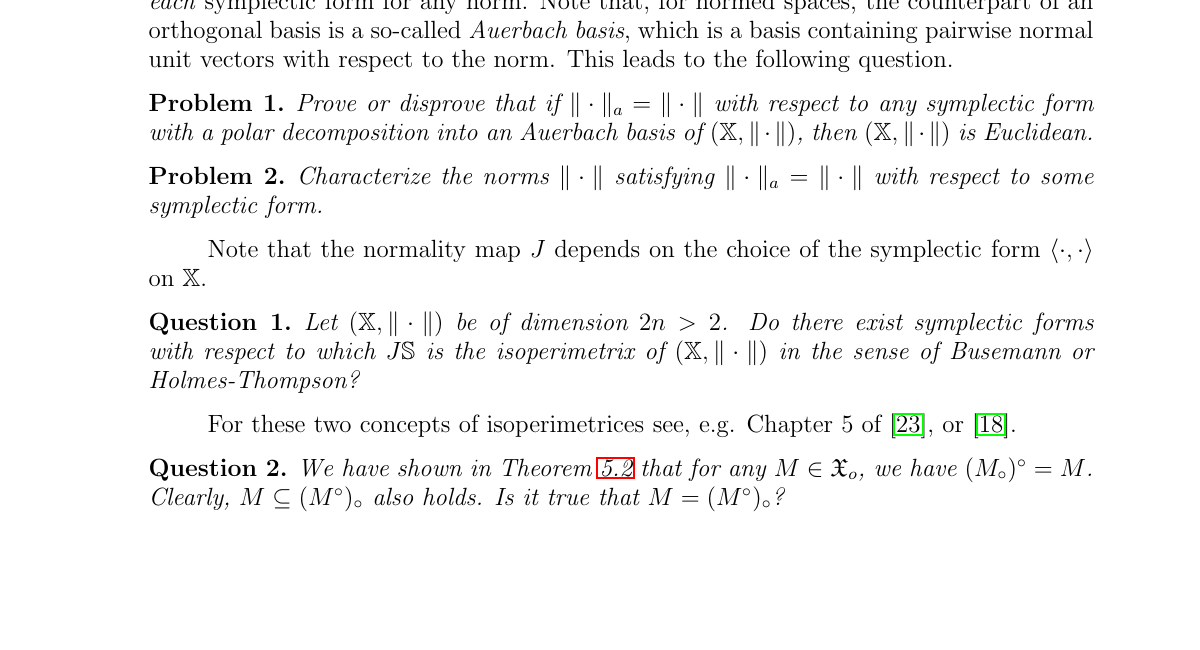
\includegraphics[width=\textwidth]{figures/open_question_page14.png}
\caption{The open question on page 14 of the source PDF.}
\label{fig:question}
\end{figure}

\section{The structural obstruction}

Write
\[
 F:X\longrightarrow X^*,\qquad F(y)(x)=[x,y].
\]
Under the standing smoothness and strict-convexity assumptions, the
generalized Riesz representation theorem recalled by the source says that
$F$ is a bijection.  It is positively and negatively homogeneous but need
not be additive.

\begin{theorem}[Convex-hull formula]\label{thm:formula}
For every convex body $M\subset X$ containing the origin in its interior,
\begin{equation}\label{eq:formula}
 (M^\circ)_\circ=F^{-1}\!\bigl(\conv F(M)\bigr).
\end{equation}
Consequently,
\[
 M=(M^\circ)_\circ \quad\Longleftrightarrow\quad F(M)\text{ is convex}.
\]
\end{theorem}

\begin{proof}
For $A\subset X^*$ and $C\subset X$, use the ordinary one-sided polars
\[
 A^*=\{x\in X:\varphi(x)\leq1\ (\varphi\in A)\},\qquad
 C^*=\{\varphi\in X^*:\varphi(x)\leq1\ (x\in C)\}.
\]
The definitions give
\[
 M^\circ=F(M)^*,
 \qquad
 (M^\circ)_\circ=\{y:F(y)\in(M^\circ)^*\}.
\]
The ordinary bipolar separation argument states that
$(A^*)^*=\cl\conv(A\cup\{0\})$.  Indeed, the inclusion from right to left
is immediate, while a point outside that closed convex hull is strictly
separated from it by evaluation at some $x\in X$; rescaling $x$ puts it in
$A^*$ and excludes the point from $(A^*)^*$.

Here $0\in M$ and $F(0)=0$.  Moreover $F$ is continuous: if $y_k\to y$,
then $\|F(y_k)\|_*=\|y_k\|$; every convergent subsequence of $F(y_k)$ has a
limit norming $y$, and uniqueness of the norming functional forces that
limit to be $F(y)$.  Thus $F(M)$ is compact, and in finite dimensions its
convex hull is compact.  Applying the bipolar identity to $F(M)$ yields
\eqref{eq:formula}.  Since $F$ is bijective, equality with $M$ holds exactly
when $\conv F(M)=F(M)$.
\end{proof}

The formula pinpoints why the source's proved order works while the reversed
one may fail: the nonlinear duality map need not carry a convex body to a
convex set.

\section{An explicit counterexample in \texorpdfstring{$\ell_4^2$}{ell-4 squared}}

Let $X=\R^2$ with the $\ell_4$ norm.  This norm is smooth and strictly
convex.  Its standard induced semi-inner product is
\begin{equation}\label{eq:sip}
 [x,z]_4=
 \frac{x_1z_1^3+x_2z_2^3}{\|z\|_4^2}
 \quad(z\ne0),
 \qquad [x,0]_4=0.
\end{equation}
Let $B_2$ denote the Euclidean unit disk, let $e_1,e_2$ be the coordinate
vectors, and set
\begin{equation}\label{eq:M}
 M=\conv\!\left(\frac1{10}B_2\cup\{e_1,e_2\}\right),
 \qquad
 y=\left(\frac1{\sqrt2},\frac1{\sqrt2}\right).
\end{equation}

\begin{theorem}\label{thm:counterexample}
The set $M$ in \eqref{eq:M} is a convex body with $0$ in its interior, and
\[
 y\in(M^\circ)_\circ\setminus M.
\]
In particular, Question~2 has a negative answer.
\end{theorem}

\begin{proof}
The inclusion $(1/10)B_2\subset M$ makes $M$ a compact convex body with
$0$ in its interior.  Consider the linear functional
$L(z)=z_1+z_2$.  Its maximum on $(1/10)B_2$ is $\sqrt2/10<1$, while
$L(e_1)=L(e_2)=1$.  Therefore $L\leq1$ throughout $M$.  But
\[
 L(y)=\sqrt2>1,
\]
so $y\notin M$.

Now let $x=(x_1,x_2)\in M^\circ$.  Since $e_1,e_2\in M$, the definition of
the right semi-polar and \eqref{eq:sip} give
\[
 x_1=[x,e_1]_4\leq1,
 \qquad
 x_2=[x,e_2]_4\leq1.
\]
For the point $y$ in \eqref{eq:M}, one has $\|y\|_4^2=2^{-1/2}$ and
$y_1^3=y_2^3=2^{-3/2}$.  Hence
\[
 [x,y]_4=\frac{x_1+x_2}{2}\leq1.
\]
This inequality holds for every $x\in M^\circ$, which is precisely the
condition $y\in(M^\circ)_\circ$.  Together with $y\notin M$, it proves the
strict inclusion.
\end{proof}

The same point can be read through Theorem~\ref{thm:formula}: formula
\eqref{eq:sip} gives $F(e_1)=(1,0)$, $F(e_2)=(0,1)$, and
$F(y)=(1/2,1/2)$.  Thus $F(y)$ lies on the segment joining two points of
$F(M)$ even though $y$ lies outside $M$.

\section{Verification, scope, and novelty}

The proof is exact and has no numerical dependency.  It uses the source's
one-sided inequalities exactly as written; in particular no symmetry of
$M$ or of the semi-inner product is assumed.  The auxiliary Euclidean disk
only ensures that $0$ is an interior point of $M$; the semi-inner product is
induced throughout by $\ell_4^2$.  The complete convention and hypothesis
audit is recorded in the companion \texttt{verification.md}.

This is a full negative answer to Question~2 and also supplies a criterion
for equality for each individual body.  It does not address the source's
other questions about antinorms, isoperimetrices, or odd-dimensional
analogues.

Before promotion, the run indexes were searched using arXiv:1308.0974, the
exact title, semi-polarity, right and left semi-polars, and the displayed
double operation.  Bounded web searches on 11 August 2026 used the exact
question, close variants, the article title and DOI, and citation-oriented
queries.  They found the source and later papers citing it for background,
but no answer to Question~2 and no matching $\ell_4^2$ construction.
Novelty confidence is moderate because citation/search coverage is bounded.

\begin{thebibliography}{9}
\bibitem{HLS}
\'A.~G.~Horv\'ath, Z.~L\'angi, and M.~Spirova,
\emph{Semi-inner products and the concept of semi-polarity},
Results Math. 71 (2017), 127--144;
arXiv:1308.0974.
\url{https://arxiv.org/abs/1308.0974}.
\end{thebibliography}

\end{document}
